\documentclass[tikz,border=5pt]{standalone}
\usetikzlibrary{positioning}
\usepackage{graphicx}
\begin{document}
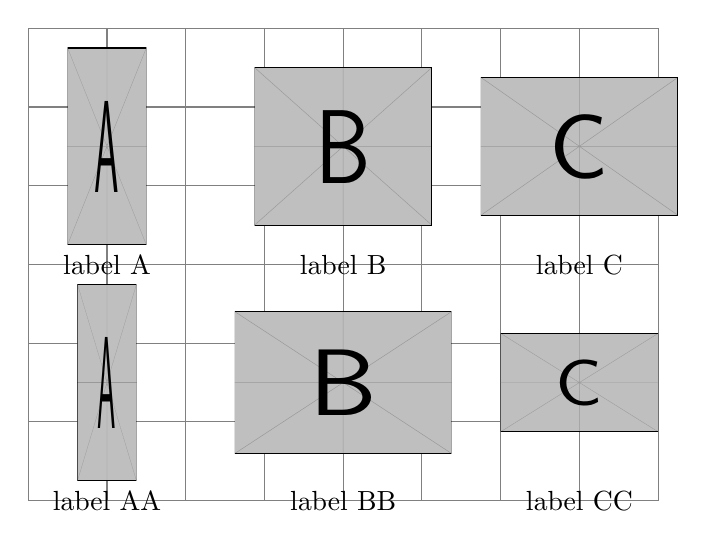
\begin{tikzpicture}
\draw[gray] (-4,-3) grid (4,3);
\node (A) at (-3,1.5) {\includegraphics[width=1cm,height=2.5cm]{example-image-a}};
\node[on grid,below=1.5cm of A] {label A};
\node (B) at (0,1.5) {\includegraphics[width=2.25cm,height=2cm]{example-image-b}};
\node[on grid,below=1.5cm of B] {label B};
\node (C) at (3,1.5) {\includegraphics[width=2.5cm,height=1.75cm]{example-image-c}};
\node[on grid,below=1.5cm of C] {label C};
\node (AA) at (-3,-1.5) {\includegraphics[width=.75cm,height=2.5cm]{example-image-a}};
\node[on grid,below=1.5cm of AA] {label AA};
\node (BB) at (0,-1.5) {\includegraphics[width=2.75cm,height=1.8cm]{example-image-b}};
\node[on grid,below=1.5cm of BB] {label BB};
\node (CC) at (3,-1.5) {\includegraphics[width=2cm,height=1.25cm]{example-image-c}};
\node[on grid,below=1.5cm of CC] {label CC};
\end{tikzpicture}

\end{document}